\documentclass{IEEEoj-data}
\usepackage{cite}
\usepackage{amsmath,amssymb,amsfonts}
\usepackage{graphicx,color}
\usepackage{textcomp}
\usepackage{hyperref}
\usepackage{balance}
\usepackage{booktabs}
\usepackage{array}
\usepackage{tabularx}
\usepackage{pgfplots}
\usetikzlibrary{positioning,arrows.meta}
\pgfplotsset{compat=1.18}
\hypersetup{hidelinks}
\def\BibTeX{{\rm B\kern-.05em{\sc i\kern-.025em b}\kern-.08em
    T\kern-.1667em\lower.7ex\hbox{E}\kern-.125emX}}
\AtBeginDocument{\definecolor{ojcolor}{cmyk}{0.93,0.59,0.15,0.02}}
\definecolor{databar}{RGB}{151,35,75}
\newcolumntype{Y}{>{\raggedright\arraybackslash}X}

\begin{document}
% Add article DOI and received/revised/accepted/publication dates when assigned.

\title{{\color{black}\textbf{Descriptor:}} \textit{The Residential 1 Hz Energy Dataset} (R1Hz)}

\author{Stephen Makonin\authorrefmark{1}, (SENIOR MEMBER, IEEE), Danielle Jaye Agron\authorrefmark{2}, (STUDENT MEMBER, IEEE), AND Patrick Palmer\authorrefmark{2}, (SENIOR MEMBER, IEEE)}
\affil{School of Engineering Science, Simon Fraser University, Burnaby, BC, Canada, V5A 1S6}
\affil{School of Mechatronic Systems Engineering, Simon Fraser University, Surrey, BC, Canada, V3T 0N1}
\corresp{CORRESPONDING AUTHOR: Stephen Makonin (e-mail: smakonin@sfu.ca).}
\authornote{This work was supported by the Natural Sciences and Engineering Research Council of Canada (NSERC) Discovery Grant RGPIN-2018-06192.}
\markboth{DESCRIPTOR: THE RESIDENTIAL 1 HZ ENERGY DATASET (R1HZ)}{MAKONIN et al.}

\begin{abstract}
The Residential 1 Hz Energy Dataset (R1Hz) contains circuit-level electrical measurements from one side-attached duplex in Burnaby, British Columbia, Canada. Four aligned 1 Hz files provide current, power factor, real power, and reactive power for one main aggregate and 18 named circuit/load channels over 757 days, from 13 September 2017 through 9 October 2019. Each file contains 65,404,800 rows. The release also contains hourly, daily, and monthly interval-energy products; native in-home-display (IHD) observations; hourly utility energy; outdoor climate observations; a channel dictionary; and daily unprocessed Modbus acquisition records retained for provenance. Two acquisition outages affected 0.203758\% of the circuit-value cells in the four 1 Hz streams. Missing circuit values were imputed deterministically from weekday- and local-clock-aligned observations 364 days away; 13 additional isolated real/reactive-power seconds were estimated from contemporaneous electrical measurements. Every row containing a synthetic value is marked \texttt{s}. This paper documents the instrumentation, exact released schemas, recovery methods, validation, remaining limitations, and storage organization needed for reproducible use of R1Hz.\\
\\
{\textcolor{ieeedata}{\abstractheadfont\bfseries{IEEE SOCIETY/COUNCIL}}} Power and Energy Society (PES)\\
\\
{\textcolor{ieeedata}{\abstractheadfont\bfseries{DATA DOI/PID}}} \href{https://doi.org/10.7910/DVN/RCB5VJ}{10.7910/DVN/RCB5VJ}\\
\\
{\textcolor{ieeedata}{\abstractheadfont\bfseries{DATA TYPE/LOCATION}}} Time series; Burnaby, British Columbia, Canada
\end{abstract}

\begin{IEEEkeywords}
energy data, imputation, load disaggregation, non-intrusive load monitoring, power measurement, residential electricity, smart meter
\end{IEEEkeywords}

\maketitle

\section*{BACKGROUND}
Public, high-resolution residential electricity datasets are important for evaluating load forecasting, anomaly detection, demand response, energy feedback, and non-intrusive load monitoring (NILM) under realistic operating conditions. Their value depends not only on sampling frequency, but also on an explicit time base, named loads, stable schemas, provenance, quality flags, and disclosure of any synthetic values.

R1Hz complements datasets that trade temporal resolution, monitoring duration, and number of sites in different ways. SmartNIALMeter includes many buildings and appliances at approximately 5 s resolution \cite{1}; Plegma combines appliance and contextual observations in Greece \cite{2}; and RAE provides an earlier Canadian residential smart-meter resource \cite{5}. Reviews of reproducible NILM research emphasize that transparent preprocessing and consistent evaluation are as important as open access \cite{3}. R1Hz contributes a continuous 1 Hz index, 19 named electrical channels, multiple electrical quantities, interval-energy derivatives, and retained native acquisition records for a single deeply monitored residence. Its purpose is detailed within-site analysis rather than population inference.

\section*{COLLECTION METHODS AND DESIGN}

\subsection{Monitoring Site and Instrumentation}
The monitored site is one side-attached duplex in Burnaby, British Columbia, in the \texttt{America/Vancouver} time zone. The dwelling was built in 2016, has two levels (approximately 105.4 and 67.5~m$^2$), and had approximately three occupants during collection. These descriptors provide context only; no occupant-level variables are released.

Branch-circuit measurements were collected with a DENT PowerScout 24 installed at the electrical panel. Twenty-one physical meter inputs were converted into 19 logical channels: \texttt{main} combines the two service legs on meters 1 and 2, and \texttt{dryr} combines the two dryer legs on meters 4 and 5. The other 17 logical channels each map to one physical input. Current, power factor, real power, and reactive power were placed on a common 1 Hz index. A Rainforest Automation Eagle 200 ZigBee gateway/in-home display (IHD) supplied native smart-meter power and cumulative-energy observations at an irregular interval of approximately 8--15 s. The release contains 1,619,689 native IHD records from 13 September 2017 through 13 September 2018. Separate hourly utility-energy records cover 9 June 2016 through 20 November 2019, and hourly outdoor climate records cover 1 September 2017 through 31 October 2019.

\begin{figure}[t]
    \centering
    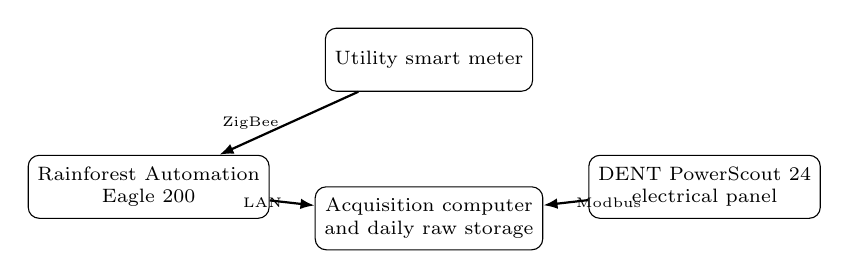
\begin{tikzpicture}[
        device/.style={draw,rounded corners,align=center,font=\scriptsize,minimum width=25mm,minimum height=8mm},
        flow/.style={-{Latex[length=1.8mm]},thick},
        node distance=8mm and 7mm]
        \node[device] (utility) {Utility smart meter};
        \node[device,below left=of utility] (eagle) {Rainforest Automation\\Eagle 200};
        \node[device,below right=of utility] (panel) {DENT PowerScout 24\\electrical panel};
        \node[device,below=12mm of utility] (computer) {Acquisition computer\\and daily raw storage};
        \draw[flow] (utility) -- node[left,font=\tiny]{ZigBee} (eagle);
        \draw[flow] (panel) -- node[right,font=\tiny]{Modbus} (computer);
        \draw[flow] (eagle) -- node[left,font=\tiny]{LAN} (computer);
    \end{tikzpicture}
    \caption{Collection architecture. The Eagle 200 receives utility smart-meter data, the PowerScout 24 measures branch circuits, and the acquisition computer stores the native records.}
    \label{fig:hardware}
\end{figure}

\subsection{Outdoor Climate Source}
Hourly meteorological observations were obtained from Environment and Climate Change Canada's Historical Climate Data service for \textit{VANCOUVER INTL A}, British Columbia (Climate Identifier 1108395; WMO Identifier 71892; Transport Canada Identifier YVR) \cite{ecccstation}. The station is listed at 49.19$^\circ$~N, 123.18$^\circ$~W and 4.30~m elevation; its current operator is NAV Canada. The word ``current'' does not imply that NAV Canada operated the station throughout the complete historical record.

The downloaded source timestamps use local standard time (PST) throughout the year. Following the source instruction, one hour was added where daylight-saving time was observed before representing the data in \texttt{America/Vancouver} local civil time. The released fields and units are: air temperature and dew point in $^\circ$C; relative humidity in percent; precipitation amount in mm; wind direction in tens of degrees true (the direction from which wind blows, with 0 denoting calm); wind speed in km/h; visibility in km; and station pressure in kPa. Humidex and wind chill are indices, and \texttt{weather} is categorical text \cite{eccctech}.

Source quality flags are not copied into separate released columns. In the source, \texttt{E} denotes estimated, \texttt{M} missing, \texttt{NA} not available, and a blank denotes an unobserved value; \texttt{D}, where present, denotes data subject to further quality control. For a NAV Canada station's \texttt{Weather} field specifically, the source FAQ explains that \texttt{NA} means no special weather elements were reported rather than an unavailable quantitative observation \cite{ecccfaq}. Redistribution follows the source site's Limited Use Software and Data Product Licence Agreement. It permits redistribution without an explicit fee for the ECCC product provided that ECCC is acknowledged and recipients accept the same redistribution restrictions; the repository's software licence does not govern the climate observations \cite{eccclicense}.

\subsection{Pre-processing and Aggregation}
The native Modbus records are retained unchanged in \texttt{raw\_modbus/}. The processed circuit streams use lowercase logical channel identifiers from \texttt{appliances.csv}. Apart from the sparse native IHD field in \texttt{power.csv}, the four 1 Hz files have the same 65,404,800 consecutive timestamps and the same 19 circuit channels. Real power and reactive power are stored as integer watts and var, current in amperes, and power factor as a dimensionless ratio.

The three interval-energy products use watt-hours. An hourly record labelled at time $T$ summarizes the preceding hour $[T-1\,\mathrm{h},T)$. Daily records group hourly labels by local date, and monthly records group daily labels by local year-month. Consequently, the first monthly record begins on 13 September 2017 and the final monthly record is a partial October 2019. Users requiring strict civil-day energy boundaries should account for this label-grouping convention and daylight-saving transitions.

\subsection{Filling Missing Data}
The original four circuit streams already contained a complete, ordered 1 Hz timestamp index: there were no absent, duplicated, reversed, or malformed timestamp rows. The missing data were blank circuit measurement fields within that index. Two outages were common to all four quantities: 8 June 2018 11:21:53 through 9 June 2018 19:35:34 PDT (116,022 s), and 1 June 2019 02:32:34 through 07:19:52 PDT (17,239 s). Thirteen additional seconds contained blanks only in real and reactive power.

The long outages were filled by deterministic, same-channel donor substitution at a 364-day offset. A 364-day shift preserves weekday and local clock time: the June 2018 outage uses 7--8 June 2019, while the June 2019 outage uses 2 June 2018. Donor intervals were checked for null circuit fields. Target timestamps and any originally observed values were retained; for example, one measured \texttt{current/gen2} value inside the first outage was not overwritten. This procedure is pattern-based imputation, not stochastic simulation, and the resulting values are plausible surrogates rather than recovered ground truth.

For the 13 isolated seconds, channel-specific real power was estimated from nearby valid observations using
\begin{equation}
    \widehat{P}_{c,t}=\widehat{\alpha}_{c}+\widehat{\beta}_{c}\bigl(I_{c,t}\,PF_{c,t}\bigr),
    \label{eq:localpower}
\end{equation}
then rounded to whole watts. Reactive power was linearly interpolated between the nearest valid bracketing observations for each channel and rounded to whole var. These methods use contemporaneous current and power factor or immediate temporal neighbours instead of an opposite-year donor when the gap is isolated.

Hourly circuit-energy gaps were reconstructed from recovered 1 Hz real power. Of 135 reconstructed utility-hour cells, 90 used the mean of at least 440 native IHD samples in the associated source hour, rounded to the utility series' 10 Wh resolution; 14 used a month-local linear model of utility energy on main energy with partial IHD available as a check; and 31 used that model without IHD coverage. Daily and monthly products were then rebuilt from the hourly product so that blanks were not silently skipped. Table~\ref{tab:imputation} gives the exact scope.

\begin{table*}[t]
\centering
\caption{Missing-data recovery in the release. Percentages for the four 1 Hz files use 65,404,800 timestamp rows or $65{,}404{,}800\times19$ circuit cells per file.}
\label{tab:imputation}
\scriptsize
\begin{tabularx}{\textwidth}{lrrrrY}
\toprule
File & Rows marked \texttt{s} & Imputed cells & Cells in scope & Imputed (\%) & Method / remaining blanks \\
\midrule
\texttt{current.csv} & 133,261 & 2,531,958 & 1,242,691,200 & 0.203748 & 364-day, same-channel donor; none remain \\
\texttt{power\_factor.csv} & 133,261 & 2,531,959 & 1,242,691,200 & 0.203748 & 364-day, same-channel donor; none remain \\
\texttt{power.csv} & 133,274 & 2,532,206 & 1,242,691,200 & 0.203768 & Donor plus local regression; none remain in circuit fields \\
\texttt{reactive.csv} & 133,274 & 2,532,206 & 1,242,691,200 & 0.203768 & Donor plus local interpolation; none remain \\
\textbf{Four-file total} & --- & \textbf{10,128,329} & \textbf{4,970,764,800} & \textbf{0.203758} & Sparse \texttt{ihd} field excluded from circuit-cell denominator \\
\midrule
\texttt{energy\_hourly.csv} & 174 & 876 & 363,360 & 0.241083 & 741 circuit and 135 utility cells; 19 first-record circuit blanks remain \\
\texttt{energy\_daily.csv} & 47 & --- & --- & --- & Rebuilt from hourly values; no energy blanks remain \\
\texttt{energy\_monthly.csv} & 21 & --- & --- & --- & Rebuilt from daily values; no energy blanks remain \\
\bottomrule
\end{tabularx}
\end{table*}

\section*{VALIDATION AND QUALITY}
Full-file scans verified the row count, schema, timestamp order, and null count of each recovered 1 Hz stream. All originally observed circuit measurements were compared with their source counterparts and were unchanged; only targeted blank cells were populated. The recovered streams contain no remaining blank circuit measurements. The sparse \texttt{ihd} column in \texttt{power.csv} is expected because it is populated only when a native IHD observation exists.

Aggregation checks compared clean observed intervals with values independently recomputed from the higher-frequency source. For 3,192 observed circuit-hour comparisons, aggregation from 1 Hz real power had a mean absolute error (MAE) of 0.263 Wh and a 95th-percentile absolute error of 1 Wh. Direct IHD aggregation had an MAE of 1.77 Wh over 3,379 observed utility hours (95th percentile 10 Wh). The month-local utility-to-main comparison had an MAE of 1.181 Wh over 9,364 observed hours (95th percentile 10 Wh). Hourly-to-daily and daily-to-monthly reconciliation after recovery both had a maximum absolute difference of 0 Wh.

Quality flags and remaining limitations must be retained in downstream analysis. The 19 blank circuit cells at the first hourly record are intentional because the preceding hour lies outside 1 Hz coverage. The source \texttt{utility.csv} contains 172 blank hourly-energy values among 30,240 rows (0.568783\%). The native \texttt{ihd.csv} includes 76 retained duplicate timestamps. Five climate hours have all observation fields blank; \texttt{precip\_amt} is blank throughout the current climate file, while humidex and wind-chill fields are conditionally applicable. The pre-existing \texttt{+} marker denotes a row added during the original time-series regularization; it occurs on 64 current/power-factor rows and 51 real/reactive-power rows and is distinct from the later recovery marker \texttt{s}. Synthetic intervals should normally be excluded from event-timing, transient, and ground-truth NILM evaluation, or included only in a clearly reported sensitivity analysis.

\section*{RECORDS AND STORAGE}
The authoritative dataset record is \href{https://doi.org/10.7910/DVN/RCB5VJ}{https://doi.org/10.7910/DVN/RCB5VJ} \cite{r1hzdata}. Table~\ref{tab:files} lists the logical release files. Counts exclude the header row. Sizes are uncompressed sizes of the canonical recovered files; compressed archive sizes will differ.

\begin{table*}[t]
\centering
\caption{Release inventory. ``1 Hz'' means one row per second; the IHD cadence is native and irregular. The raw directory contains 757 daily files.}
\label{tab:files}
\scriptsize
\begin{tabularx}{\textwidth}{l l r l r Y}
\toprule
Logical path & Grain & Data rows & Coverage (local time) & Size & Description \\
\midrule
\texttt{appliances.csv} & dictionary & 19 & not applicable & 895 B & Logical-channel names, physical meter mapping, and mixed-load notes \\
\texttt{climate.csv} & hourly & 18,984 & 2017-09-01--2019-10-31 & 1.271 MiB & Outdoor temperature, humidity, wind, pressure, visibility, and condition fields \\
\texttt{current.csv} & 1 Hz & 65,404,800 & 2017-09-13--2019-10-09 & 6.581 GiB & Circuit current (A) \\
\texttt{power\_factor.csv} & 1 Hz & 65,404,800 & 2017-09-13--2019-10-09 & 7.736 GiB & Circuit power factor (dimensionless) \\
\texttt{power.csv} & 1 Hz & 65,404,800 & 2017-09-13--2019-10-09 & 4.768 GiB & Circuit real power (W) and sparse aligned IHD power \\
\texttt{reactive.csv} & 1 Hz & 65,404,800 & 2017-09-13--2019-10-09 & 4.604 GiB & Circuit reactive power (var) \\
\texttt{energy\_hourly.csv} & hourly & 18,168 & 2017-09-13--2019-10-09 & 1.457 MiB & Utility, main, and circuit interval energy (Wh) \\
\texttt{energy\_daily.csv} & daily & 757 & 2017-09-13--2019-10-09 & 81.546 KiB & Daily-labelled energy aggregates (Wh) \\
\texttt{energy\_monthly.csv} & monthly & 26 & 2017-09--2019-10 & 3.724 KiB & Monthly-labelled energy aggregates (Wh); edge months are partial \\
\texttt{ihd.csv} & native 8--15 s & 1,619,689 & 2017-09-13--2018-09-13 & 67.954 MiB & Native IHD power (W) and cumulative meter energy (kWh) \\
\texttt{utility.csv} & hourly & 30,240 & 2016-06-09--2019-11-20 & 1.039 MiB & Native utility interval energy (Wh, 10 Wh resolution) \\
\texttt{raw\_modbus/SUB\_YYYY-MM-DD.csv} & one local day/file & typically 691,200/file & 2017-09-13--2019-10-09 & 76.711 GiB total & Headerless, immutable device-native Modbus register records; 757 files \\
\bottomrule
\end{tabularx}
\end{table*}

The four uncompressed 1 Hz CSVs exceed the Harvard Dataverse 2.5 GB per-file limit. They may therefore be distributed as compressed archives or as date-partitioned compressed members. The raw files may likewise be grouped into documented archives. Archive member names should preserve the logical names in Table~\ref{tab:files}; a release manifest should record each member's date range, uncompressed byte count, row count, and checksum. If a compressed member still exceeds the repository limit, partitioning by documented contiguous date ranges is preferable to opaque multipart archives.

The \texttt{raw\_modbus/} directory forms the provenance and audit layer. It contains one file for every local date in the 757-day acquisition interval, totalling 82,367,715,595 bytes (76.711 GiB). Each headerless \texttt{SUB\_YYYY-MM-DD.csv} contains 45 fields: a Unix timestamp, a register-bank identifier \texttt{A}--\texttt{H}, and 43 raw integer values corresponding in order to Modbus holding registers 4021--4063. A complete ordinary day has eight bank rows for each of 86,400 seconds, or 691,200 rows. Counts can differ when a day is partial or daylight-saving time changes; for example, the partial 9 June 2018 file has 126,912 rows and the 4 November 2018 fall-back file has 720,000 rows. These files are not imputed or normalized. The root-level processed files are derived data products. Retaining both layers allows users to audit register conversion, channel mapping, timestamp treatment, and recovery without mistaking synthetic values for device observations.

\subsection{Temporal Fields and Markers}
\texttt{unix\_ts} is an integer Unix timestamp in seconds with UTC as its reference. \texttt{date}/\texttt{time} and \texttt{local\_dt}/\texttt{local\_tm} are local civil-time representations in \texttt{America/Vancouver}. The \texttt{span} field is \texttt{H}, \texttt{D}, or \texttt{M} for hourly, daily, or monthly aggregates. Daylight-saving placeholders and retained native duplicates mean that \texttt{unix\_ts} is not globally unique in every auxiliary file; users should interpret it together with \texttt{marker}. Table~\ref{tab:markers} documents all marker values present in the release.

\begin{table}[t]
\centering
\caption{Marker values used in released CSVs.}
\label{tab:markers}
\scriptsize
\begin{tabularx}{\columnwidth}{cY}
\toprule
Marker & Meaning \\
\midrule
blank & Ordinary record with no special provenance flag \\
\texttt{+} & Row added during the original 1 Hz time-series regularization. This legacy flag is retained separately from later imputation. \\
\texttt{s} & At least one value in the row is synthetic/imputed. In daily or monthly energy, at least one lower-grain input is synthetic. \\
\texttt{d} & Retained duplicate native timestamp in \texttt{ihd.csv} \\
\texttt{t} & Local-time discontinuity associated with a daylight-saving-time transition in hourly utility/climate series \\
\bottomrule
\end{tabularx}
\end{table}

\subsection{Logical Electrical Channels}
The channel dictionary in Table~\ref{tab:4} replaces generic and incorrect \texttt{sub?} labels. A ``mixed'' channel can contain more than one end use and is not appliance-level ground truth.

\begin{table*}[t]
\centering
\caption{Processed logical channel dictionary. Meter numbers refer to PowerScout physical inputs.}
\label{tab:4}
\scriptsize
\begin{tabularx}{\textwidth}{l l l c Y}
\toprule
ID / CSV field & Meter input(s) & Description & Mixed & Notes \\
\midrule
\texttt{main} & 1+2 & House sub-panel & Y & Utility also supplies an unmetered garage load outside this sub-panel \\
\texttt{beda} & 13 & Bedroom plugs & Y & AFCI arc-fault plugs \\
\texttt{bedp} & 6 & Bedroom plugs & Y & --- \\
\texttt{boil} & 8 & Boiler & N & Hot water and radiant heating \\
\texttt{chrg} & 21 & Phone chargers & N & Garburator and microwave were not installed \\
\texttt{cwsh} & 10 & Clothes washer & N & --- \\
\texttt{dryr} & 4+5 & Clothes dryer & N & Two electrical legs combined \\
\texttt{dwsh} & 19 & Dishwasher & N & --- \\
\texttt{frdg} & 11 & Kitchen refrigerator & N & --- \\
\texttt{gen1} & 3 & Lights and plugs & Y & General circuit \\
\texttt{gen2} & 9 & Lights and plugs & Y & General circuit \\
\texttt{gen3} & 12 & Lights and plugs & Y & Includes Internet/network equipment \\
\texttt{gen4} & 16 & Lights and plugs & Y & General circuit \\
\texttt{gen5} & 17 & Lights and plugs & Y & General circuit \\
\texttt{gen6} & 20 & Lights and plugs & Y & General circuit \\
\texttt{kit1} & 14 & Kitchen counter plugs & Y & --- \\
\texttt{kit2} & 15 & Kitchen counter plugs & Y & --- \\
\texttt{outp} & 18 & Outside plugs & Y & --- \\
\texttt{vacu} & 7 & Built-in vacuum & N & --- \\
\bottomrule
\end{tabularx}
\end{table*}

\subsection{Exact CSV Schemas}
Table~\ref{tab:schemas} gives the ordered fields rather than unsupported generic \texttt{sub1}--\texttt{sub24} columns. All processed electrical identifiers are lowercase. For compactness, $\mathcal{C}$ denotes the 19 ID/CSV fields in Table~\ref{tab:4}, in the exact top-to-bottom order shown there.

\begin{table*}[t]
\centering
\caption{Ordered schemas of the released CSV files. Here $\mathcal{C}$ is the ordered 19-channel sequence defined above.}
\label{tab:schemas}
\scriptsize
\begin{tabularx}{\textwidth}{lY}
\toprule
File(s) & Ordered columns \\
\midrule
\texttt{appliances.csv} & \texttt{appliance\_id, name, meter\_l1, meter\_l2, is\_mains, has\_mixed\_loads, notes} \\
\texttt{climate.csv} & \texttt{unix\_ts, marker, local\_dt, local\_tm, temp, dew\_point, rel\_hum, precip\_amt, wind\_dir, wind\_spd, visibility, stn\_press, hmdx, wind\_chill, weather} \\
\texttt{current.csv}, \texttt{power\_factor.csv}, \texttt{reactive.csv} & \texttt{unix\_ts, marker, date, time}, followed by $\mathcal{C}$ \\
\texttt{power.csv} & \texttt{unix\_ts, marker, date, time, ihd}, followed by $\mathcal{C}$ \\
\texttt{energy\_hourly.csv}, \texttt{energy\_daily.csv}, \texttt{energy\_monthly.csv} & \texttt{unix\_ts, span, marker, local\_dt, local\_tm, utility}, followed by $\mathcal{C}$ \\
\texttt{ihd.csv} & \texttt{unix\_ts, marker, date, time, power, energy} \\
\texttt{utility.csv} & \texttt{unix\_ts, marker, local\_dt, local\_tm, energy} \\
\texttt{raw\_modbus/SUB\_YYYY-MM-DD.csv} & Headerless: \texttt{unix\_ts}, bank identifier \texttt{A}--\texttt{H}, then 43 integer register values for addresses 4021--4063 in ascending order \\
\bottomrule
\end{tabularx}
\end{table*}

\section*{INSIGHTS AND NOTES}

\subsection{Energy Composition}
The recovered monthly product totals 6,804.210 kWh at the utility meter and 6,671.084 kWh at the monitored house sub-panel. The 18 non-main logical channels sum to 6,547.487 kWh. These quantities are related but not interchangeable: the utility meter includes a garage load that is outside the monitored sub-panel, and circuit sums can differ from \texttt{main} because of metering coverage, instrument accuracy, rounding, and synthetic recovery. Figure~\ref{fig:energy} therefore excludes both utility and main from the component composition and reports them separately in the text.

\begin{figure}[!t]
\centering
\begin{tikzpicture}
\begin{axis}[
    xbar,
    width=0.90\columnwidth,
    height=0.34\textheight,
    bar width=5pt,
    xmin=0,
    xmax=2300,
    xlabel={Energy over the released interval (kWh)},
    symbolic y coords={Phone chargers,Outside plugs,Vacuum,Clothes washer,Dishwasher,Kitchen counter,Boiler,Kitchen refrigerator,Clothes dryer,Bedroom plugs,Lights/plugs},
    ytick=data,
    yticklabel style={font=\scriptsize},
    xticklabel style={font=\scriptsize},
    nodes near coords,
    nodes near coords style={font=\tiny},
    every axis plot/.append style={fill=databar!55,draw=databar},
    enlarge y limits=0.05,
    grid=major,
    grid style={gray!20}
]
\addplot coordinates {
    (3.380,Phone chargers)
    (19.369,Outside plugs)
    (36.602,Vacuum)
    (119.028,Clothes washer)
    (184.287,Dishwasher)
    (205.503,Kitchen counter)
    (726.626,Boiler)
    (952.857,Kitchen refrigerator)
    (1063.579,Clothes dryer)
    (1436.466,Bedroom plugs)
    (1799.790,Lights/plugs)
};
\end{axis}
\end{tikzpicture}
\caption{Non-overlapping component energy from the 18 non-main logical channels, grouped by description. Values are kWh. The utility and \texttt{main} aggregates are deliberately excluded to avoid double counting downstream circuits.}
\label{fig:energy}
\end{figure}

\subsection{Recommended Use}
R1Hz supports circuit-load characterization, short-horizon forecasting, cross-meter comparison, missing-data research, and NILM experiments in which \texttt{main} is the aggregate and selected non-mixed circuits provide submeters. It does not provide appliance state labels, occupancy labels, or a representative sample of Canadian households. Mixed-load circuits should not be treated as single appliances. Researchers should publish the exact time range, channel set, treatment of daylight-saving time, and treatment of \texttt{s}-marked rows used in each experiment.

The native \texttt{ihd.csv}, aligned sparse \texttt{ihd} field in \texttt{power.csv}, and hourly \texttt{utility.csv} have different sampling semantics. They should not be filled or resampled implicitly. Similarly, recovered long-gap values preserve daily and weekly timing patterns but cannot reproduce the actual appliance events that occurred during the outages.

\section*{SOURCE CODE AND SCRIPTS}
The versioned collection, processing, recovery, and validation code is maintained at \href{https://github.com/smakonin/R1Hz.dataset}{github.com/smakonin/R1Hz.dataset}. The repository includes the deterministic recovery scripts, method inputs for the isolated estimates, a cell-level recovery log, validation summaries, SQL schemas, and the manuscript source. The Harvard Dataverse DOI remains the canonical citation for the data; the Git commit used for a study should additionally be recorded to identify the exact processing implementation.

\section*{ETHICS STATEMENT}
The measurements originate from a private residence and can reveal patterns of household activity even though no names, utility account identifiers, audio, images, or exact street address are released. Location is reported only at city level. Users should not attempt to re-identify residents or infer sensitive household behaviour beyond the scientific purpose of their study.

\section*{ACKNOWLEDGEMENTS AND INTERESTS}
\textit{Author contributions:} S.M. curated the data. D.J.A. and S.M. analyzed the data. D.J.A., S.M., and P.P. reviewed the content and contributed to the manuscript. All authors reviewed the manuscript.

\textit{Funding:} This work was supported by the Natural Sciences and Engineering Research Council of Canada (NSERC) Discovery Grant RGPIN-2018-06192.

\textit{Competing interests:} The authors declare no competing interests.

\balance
\bibliographystyle{IEEEtran}
\bibliography{ref}
\end{document}
